Bitwarden es un administrador de contraseñas código abierto en la nube, donde se guardan los credenciales de las distintas \glspl{cuenta} del usuario. Se accede a la base de datos desde los distintos clientes:
\begin{itemize}
    \item Escritorio
    \item Web
    \item Extensión de navegador
    \item \gls{cli}
    \item \textbf{App de Android}
    \item App de iOS
\end{itemize}

\begin{figure}[H]
    \centering
    
\includegraphics[width=\textwidth]{gfx/bitwarden-logo-horizontal.png}
    \caption{Logo de Bitwarden. \href{https://github.com/bitwarden/brand}{Realizado por Bitwarden.}}
    \label{fig:bitlogo-horizontal}
\end{figure}

Una vez en un cliente el usuario puede crear una \gls{vault} donde almacenar los credenciales de inicio de sesión en distintos servicios.
Los clientes de Bitwarden almacenan una caché de la \gls{vault} para así poder acceder a ella incluso cuando no pueden conectarse al servidor \cite{bitcache}.
Todo esto ocurre bajo un método de conocimiento cero \gls{e2ee}, y los credenciales sólo son descifrados en memoria.
Existen distintos tipos de servidores Bitwarden:
\begin{itemize}
    \item Servidor oficial: Servidor de la propia empresa Bitwarden.
    \item Self-host: Alojar una estancia manualmente en un servidor propio.
    \item \textbf{Vaultwarden}: Implementación de la \gls{api} de los servidores de Bitwarden en Rust, \textit{self-host}.
\end{itemize}

\begin{figure}[H]
    \centering
    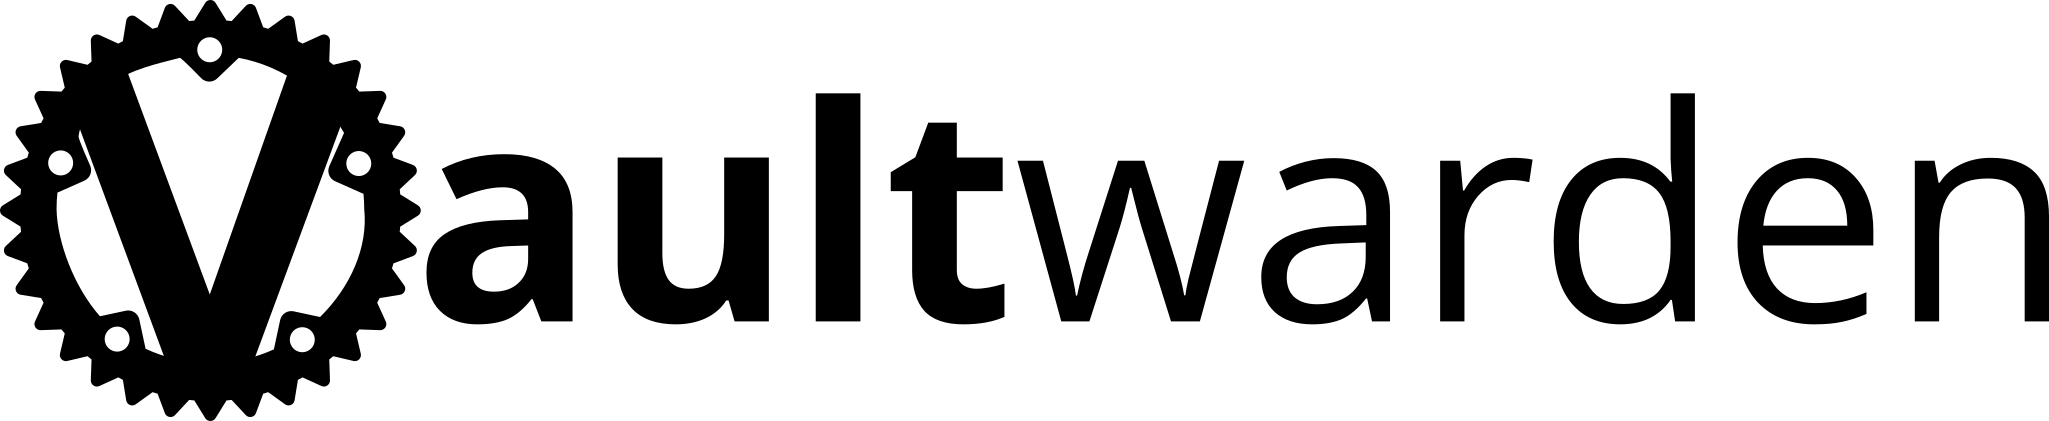
\includegraphics[width=\textwidth]{gfx/vaultwarden-logo.png}
    \caption{Logo de Vaultwarden. \href{https://vaultwarden.discourse.group/}{Realizado por Vaultwarden.}}
    \label{fig:vaultlogo}
\end{figure}

Para este proyecto se modificará la app de Android y se usará como servidor una estancia en red local de Vaultwarden.